\documentclass[12pt]{report}
%\documentclass[12pt,twoside]{report}
\usepackage[utf8]{inputenc}
\usepackage[english]{babel}
\usepackage{csquotes}
\usepackage{amssymb}
\usepackage{amsmath}
\usepackage{mathrsfs}
\usepackage{tikz}
\usepackage{forest}
\usepackage{pgfplots}
\usepackage{rotating}
\pgfplotsset{compat=1.7}
\usepackage[a4paper,width=130mm,top=45mm,bottom=45mm]{geometry}
%\usepackage[a4paper,left=3cm,right=2cm,top=2.5cm,bottom=2.5cm]{geometry}
\usepackage{marginnote}
\usepackage[makeroom]{cancel}
\usepackage[ruled,vlined,linesnumbered]{algorithm2e}
\usepackage{algorithmic}
\usepackage{graphicx}



\graphicspath{ {./images/} }

\usepackage[
    backend=biber,
    style=alphabetic,
    sorting=ynt
]{biblatex}




\addbibresource{mybib.bib} %Imports local bibliography file


%IN caso stampa in un file a parte il titolo, per allineamento amrgini destro e sinistro

%\date{ }

\begin{document}

\numberwithin{equation}{section}

\thispagestyle{empty}
%\begin{titlepage}
\vspace*{-1.5cm} \bfseries{
\begin{center}
  \large
  POLITECNICO DI MILANO\\
  \normalsize
  Corso di Laurea \textbf{MAGISTRALE} in Ingegneria Informatica\\
  Dipartimento di Elettronica e Informazione\\
  \begin{figure}[htbp]
    \begin{center}
      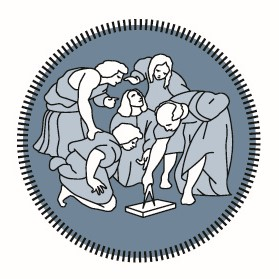
\includegraphics[width=3.5cm]{./pictures/logopm.jpg}
%	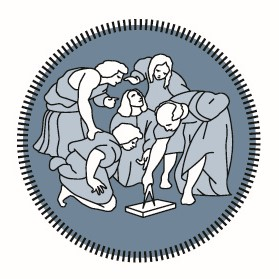
\psfig{file=./pictures/logopm.jpg,width=3.5cm}
    \end{center}
  \end{figure}
  \vspace*{0.3cm} \LARGE



  \textbf{A SURVEY ON SHORT-RANGE RSSI-BASED GEOLOCALIZATION}\\



%  \vspace*{.75truecm} \large
%  AI \& R Lab \\
%  Laboratorio di (??) Intelligenza Artificiale \\
%  e Robotica del Politecnico di Milano
\end{center}
\vspace*{3.0cm} \large
\begin{flushleft}


  Relatore: Prof. Lorenzo Mario Fagiano \\
  %Correlatore: ?? 

\end{flushleft}
\vspace*{1.0cm}
\begin{flushright}


  Tesi di Laurea di:\\ Alberto Tiraboschi, matricola 920775 \\


\end{flushright}
\vspace*{1cm}
\begin{center}



  Anno Accademico 2020-2021
\end{center} \clearpage
}
\thispagestyle{empty}  \normalfont \cleardoublepage
\newpage



\clearpage % end title page
\begingroup
  \thispagestyle{empty}
  \null
  \newpage
%  \null
%  \newpage
\endgroup


\thispagestyle{empty}
\tableofcontents
\thispagestyle{empty}

\clearpage % end title page
\begingroup
  \thispagestyle{empty}
  \null
  \newpage
%  \null
%  \newpage
\endgroup


\setcounter{page}{1}

\chapter{Introduction}
Finding the location of unknown objects has been since a long time a topic under investigation. The applications are vast and span many different topics, from security, to discover unauthorized intrusions, to warfare, to discover nearby opponents, or detecting submarines, but also to localize someone who needs to be rescued, for example in disaster response. With the recent advances in technology it has been possible to locate objects with low-cost technology, and available to almost every person in the world, Wi-Fi. The main purpose of this thesis is to tidy up a little the actual state of the art of the RSSI-based localization algorithms. Here I will do a revisitation of the most important algorithms, trying to mediate from theory to application, without losing mathematical accuracy, by adapting the theoretical concepts in a form that is ready to implement algorithmically in whichever language it is preferred. I will also add at the top of the description of each algorithm which are the parameters that one needs to know beforehand.

\section{Environment settings}
The main setting that will be presented is the most commonly used up to now, which is a space filled with receiving/transmitting devices (anchor nodes), each placed in a regular position (usually a grid) with known positions, that can read the signal intensity of the other nodes. The activity starts when a device with an unknown position is put in the area and many (if not every) nodes are close enough to get the signal intensity of that unknown node. This range of sensitivity can be seen as a circle of radius of about $50$ meters. At this point, each anchor node can communicate outside a tuple like this $(x_i,y_i,\upsilon_i^u)$ where $x_i,y_i$ are the position of the node itself, and $\upsilon_i^u$ is the signal strength intensity of the unknown node, measured by the anchor node $i$. Usually, the data is sent to a central processing device that makes the computations and outputs the estimated position. \\\\
This is not the only way however, the other way, which is lately becoming increasingly used is the employment of a drone, that given some bounds on the area to scan, it collects and outputs the samples, behaving as a ``moving" anchor node.

\clearpage

\chapter{Mathematical model of RSSI propagation}
\section{Path loss model}
Given a transmitting device $j$ and a receiving device $i$, placed at distance $d_i^j$ to one another, the receiver device can measure the signal intensity $\upsilon_i^j$ of the transmitting device. Those readings (according to the log-normal propagation model  \cite{MUNOZ200923}) are of the form
\begin{equation}
\upsilon_i^j = \upsilon_0^j-10\alpha\log_{10}\bigg(\frac{d_i^j}{d_0}\bigg) + \xi_i, \quad d_i^j>d_0
\label{eq:1}
\end{equation}
\begin{equation}
    d_i^j=\sqrt{(x_i-x_j)^2+(y_i-y_j)^2}
\end{equation}
where $\xi_i$ is a zero-mean gaussian variable ($\mathcal{N}(0,\sigma^2_i)$) that represents the noise, $\alpha$ is the path loss index, which can vary between $2$ (open field) and $4$ (environment fitted with obstacles) and $\upsilon_0^j$ is the RSSI read at $d_0$. Commonly $d_0$ is taken as $1$ meter, so that we can simplify, the \ref{eq:1} as:
\begin{equation}
\upsilon_i = \upsilon_0-10\alpha\log_{10}(d_i) + \xi_i, \quad d_i>d_0
\label{eq:2}
\end{equation}
where the letter $j$ is usually dropped.
Some algorithms don't require high precision, so they usually don't take into account the noise, whereas for some others it is necessary to rewrite the model as follows
\begin{equation}
\upsilon_i= \upsilon_0-\beta\ln(d_i) + \xi_i
\end{equation}
with
\begin{itemize}
    \item $\beta=10\alpha/\ln(10)$
    \item $\ln(\bullet)\quad \text{as the natural logarithm}$
\end{itemize}
and then deriving
\begin{equation}
\nu_i = \upsilon_i-\upsilon_0= -\beta\ln(d_i) + \xi_i
\label{eq:5}
\end{equation}
\clearpage

\chapter{Disturbances of RSSI}
The RSSI noise has a great influence over the measurements, thereby complicating the attempt to get a precise location. To give some numbers, the theoretical range within the RSSI can vary goes from $-30$ to $-120$ however the available range of signal intensity that a common WiFi device can measure varies in the interval $-30\div-90$ dbm. This is because to establish a connection (and to retrieve at least the name of the transmitting device), some packets must be sent, and if the signal strength is too low, the quality of the packets degrades, therefore making impossible communication. The value measured at the receiving end includes also the noise, so the measurement deviates from the exact value generally by at most $6$ dbm which is as much as $10\%$ over the range of measurement.
Due to its significant influence, this issue has been investigated many times to discover something more, for example about its probability distribution, but up to now, few to no answers have been found. To cite one, \cite{4608603} showed that there are no significant patterns over the time domain neither in the frequency domain. The causes of the noise are the same that affect the propagation of any electromagnetic wave. We can summarize the main sources of noise in the following sections: 
\section{Multipath Fading} 
As outlined in \cite{onl11}, multipath fading occurs when there are multiple ways for the signal to reach the receiving device. This causes the signal waves to reach the receiving end at two different times, that is, there is a non-negligible delay between the time of arrival of the two (or more) waves. This means phase shifting, leading to constructive/destructive interference, therefore causing oscillations in the signal intensity read. This effect is very preeminent in closed environments when there are many surfaces able to reflect the signal. It is totally random \cite{10.5555/559977} which means unpredictable by definition. Due to its nature, the alterations of the signal caused are like spikes above or below the mean value. Therefore it can be removed to some extent by filtering the outliers with some of the methods presented later.
\section{Shadow Fading}
This effect is the attenuation of the signal caused by heavy and large (w.r.t. the wavelength) obstacles between the receiver and the sender that can adsorb the waves partially, or even totally. This is directly related to NLOS (Non-Line Of Sight) environments that is, when the receiver cannot "see directly" the sender. The shadow fading effect is taken into account in the model as the path loss index $\alpha$. This parameter is easily obtained in an open field with no obstacles, whereas it is quite a problem when some obstacles are obstructing the way. In the latter case, the analytical way (by considering the absorption coefficients of the obstacles) is rarely used, instead, a somehow correct path loss index is usually estimated with some algorithms, one of them is presented later.\\\\ 
It showed spatial correlation \cite{244122,732812}, which is intuitive, all the measurements taken in a certain position, with a certain number of obstacles will be all affected by an almost equal shadow fading, whereas in another location it will not. The problematic effect of this noise is that it shows a systematic behavior, in other words, each measurement is affected by an almost equal amount, therefore trying to remove it by removing outliers is not an effective way. If the path loss index is taken wrong in the model for some reason, the estimated position will be altered with some significant errors, that may invalidate the improvements taken to reduce the other sources of noise. Even more complicated is when there are persons moving freely between the sender and the receiver. The body of each passing person adsorbs the signal, therefore altering the measure. The estimated position will bear some non-negligible errors.

\chapter{Noise removal}
Here I will present some algorithms to remove outliers in a series of data. Those methods, given their independence from the RSSI can be used to remove outliers of any series of data.
\subsection{IQR}
This method, whose name is InterQuartile Range, is based, as the name suggests, on the quartiles of a dataset. First, let's start with an algorithm that can be used to obtain the quartiles. I will assume some facts:
\begin{itemize}
    \item Arrays index starts from zero
    \item Float numbers are cast to integer with truncation of the decimal part, e.g.
    $$1.2 \to 1$$
    $$-1.8 \to -1$$
    \item Datasets
    \begin{itemize}
        \item d1
        \item d2
        \item d3
    \end{itemize}
    \item Size of each dataset
    \begin{itemize}
        \item s1
        \subitem size of d1
        \item s2
        \subitem size of d2
        \item s3
        \subitem size of d3
    \end{itemize}
\end{itemize}

\begin{algorithm}[H]
\SetAlgoLined
\KwResult{Q1, Q2, Q3}
d1.sort(ascending)\;
Q1 = Q2 = Q3 = 0\;
s1 = d1.size()\;
\eIf{s1 is even}{
    Q2 = (d1[s1/2 - 1] + d1[s1/2])/2\;
    d2 = d1[0 : s1/2 - 1]\;
    d3 = d1[s1/2 : s1 - 1]\;
}{
    Q2 = d1[s1/2]\;
    d2 = d1[0 : s1/2 - 1]\;
    d3 = d1[s1/2 + 1 : s1 - 1]\;
}

s2 = d2.size()\;
s3 = d3.size()\;
\eIf{s2 is even}{
    Q1 = (d2[s2/2 - 1] + d2[s2/2])/2\;
}{
    Q1 = d2[s2/2]\;
}
\eIf{s3 is even}{
    Q3 = (d3[s3/2 - 1] + d3[s3/2])/2\;
}{
    Q3 = d3[s3/2]\;
}
 \caption{Quartiles computation}
\end{algorithm}
\noindent \\A little explanation here is required. At the beginning, the algorithm sorts the initial dataset $d1$ in ascending order. We will take the median ($Q2$) of $d1$. Therefore we have two possible paths. If $s1$, size of $d1$ is odd, then the median is at $s1/2$, the central position (remind the assumption about array indexing and decimal casting). If it is not, the median will be the average of the two elements at the center. Either the cases, we get two datasets, the upper half ($d2$) and the lower half ($d3$), separated by the median. Then the operation is repeated for each one of $d2,d3$, to obtain $Q1$ median of the upper half, and $Q3$ median of the lower half. As can be seen, $25\%$ of data is below $Q1$, $50\%$ of data is below $Q2$, which is the common median, and $75\%$ of data is below $Q3$. \\\\Going back to the IQR method the algorithm goes through the following steps:

\begin{algorithm}[H]
\SetAlgoLined
\KwResult{The filtered dataset}
Q1, Q2, Q3 known from the previous algorithm\;
IQR = Q3 - Q1\;
$I=[Q1-1.5\cdot IQR,\quad Q2 + 1.5\cdot IQR]$\;
k = 0\;
 \While{iter $ \in [0:n-1]$}{
    \If{! $dataset[k]\in I$}{
        dataset.remove(k)\;
        k = k - 1\;   
  }
    k = k + 1\;
    iter = iter + 1\;
 }
 \caption{Outliers removal with IQR}
\end{algorithm}
\noindent \\Here it is given a numeric example. Suppose you have the following dataset 
$$
\text{dataset}=\begin{bmatrix}
-1.9\\ 
0.3\\ 
3.7\\
4.1\\
6\\
6.1\\
7.2\\
9\\
19
\end{bmatrix}
$$
already sorted, where the first seven numbers are extracted from $-2+X$, where $X$ follows the uniform distribution in $[0,10]$. The latest two values are possible outliers. Since the size of the dataset is odd, $Q2$ can be found at the fifth position and is $6$. We have then the first half and the second half. Since the first half has an even number of data points, the median of the first half ($Q1$) will be $(0.3+3.7)/2=2$, the same reasoning applies to $Q3$ for the second half, which is equal to $8.1$. Therefore the IQR will be $8.1-2=6.1$ the interval $I$ will be
$$I=[2-1.5\cdot6.1,8.1+1.5\cdot6.1]=[-7.15,17.25]$$
As you can see, the number $19$ will be treated as an outlier and thus be removed. You can also choose how wide the interval you want it to be, for example, if you wanted to be more strict you could choose $1$ instead of $1.5$ as a multiplying factor, obtaining the following interval
$$I'=[2-1\cdot6.1,8.1+1\cdot6.1]=[-4.1,14.2]$$

\subsection{Z-score}
The Z-score is another method to find outliers. The procedure estimates the sample mean and sample standard deviation as follows
\begin{equation}
    \hat{\mu}=\frac{1}{n}\sum_{i=1}^nx_i
\end{equation}
\begin{equation}
    \hat{\sigma}=\sqrt{\frac{1}{n-1}\sum_{i=1}^n(x_i-\hat{\mu})^2}
\end{equation}
Then it computes the z-score $y_i$ of each value $x_i$
\begin{equation}
    y_i=\frac{x_i-\hat{\mu}}{\hat{\sigma}}
\end{equation}
The filtering process now removes every data whose z-score is outside the interval $[-3,3]$. \\\\
Here an example, with the same dataset of the previous algorithm
$$
\text{dataset}=\begin{bmatrix}
-1.9\\ 
0.3\\ 
3.7\\
4.1\\
6\\
6.1\\
7.2\\
9\\
19
\end{bmatrix}
$$
The estimated mean is $\hat{\mu}=5.94$ and the sample standard deviation is $\hat{\sigma}=5.95$. Then the corresponding set of z-scores is
$$
\text{z-scores}=\begin{bmatrix}
-1.32\\
-0.95\\
-0.38\\
-0.31\\
0.01\\
0.03\\
0.21\\
0.51\\
2.19
\end{bmatrix}
$$
note the last value, for the previous algorithm it should have been discarded, but according to this one, it is still kept. Clearly, you can choose a narrower interval than $[-3,3]$ if you want to be more strict on the outliers.

\clearpage

\chapter{Algorithms for parameters estimation}
\section{Estimation of path loss index $\alpha$}
  \begin{center}
  \textbf{Assume to know:}
  \begin{itemize}
    \centering
    \item $\upsilon_0$
    \item $\xi_i,\forall i$
    \item $d_i^j,\forall i$
  \end{itemize}
  \end{center}
  Place a transmitting device $j,j>n$ at known position. For the anchor node $i,1\leq i\leq n$, the values of signal intensity of the node $j$ are obtained according to \ref{eq:2}. The referenced model is basically a constant term $[\upsilon_0-10\alpha\log_{10}(d_i)]$ added to a zero mean gaussian variable $[\xi_i]$, so from \cite{alma9926534668905776}, let $a \in \mathbb{R}$
\begin{equation}
a+\mathcal{N}(0,\sigma^2)\sim\mathcal{N}(a,\sigma^2)
\end{equation} therefore the \ref{eq:2} is gaussian as follows:
\begin{equation}
    X_i\sim \mathcal{N}(\mu_i,\sigma^2_i)
    \label{eq:3}
\end{equation}
where 
\begin{equation}
    \mu_i = \upsilon_0-10\alpha\log_{10}(d_i)
\end{equation}
which has probability density function
\begin{equation}
    p_i(x)=\frac{1}{\sqrt{2\pi\sigma_i^2}}e^{-\frac{1}{2}\frac{(x-\mu_i)^2}{\sigma^2_i}}
\end{equation} 
Given a sample of $n$ measurements $$\upsilon_1,...,\upsilon_n$$ one for each node, where each $\upsilon_i$ follows \ref{eq:3}. Then we can employ the Maximum Likelihood to estimate the path loss index. It follows
\begin{equation}
    L_n(\alpha,\sigma_1^2,...,\sigma_n^2)=\prod_{i=1}^nP(X_i=\upsilon_i)=
    \frac{1}{(2\pi)^{\frac{n}{2}}(\prod_{i=1}^n\sigma_i^2)^\frac{1}{2}}e^{-\frac{1}{2}\sum_{i=1}^n\frac{(\upsilon_i-\mu_i)^2}{\sigma^2_i}}
\end{equation}
by applying the logarithm to both members
\begin{equation}
    \ell_m(\alpha,\sigma_1^2,...,\sigma_n^2)=-\frac{n}{2}\ln(2\pi)-\frac{1}{2}\ln\bigg(\prod_{i=1}^n\sigma^2_i\bigg)-\frac{1}{2}\sum_{i=1}^n\frac{(\upsilon_i-\mu_i)^2}{\sigma^2_i}
\end{equation}
Maximizing $\ell_n^i$ w.r.t to $\alpha$ is equal to finding the stationary point of the third term in the above equation since the first and second one are independent from $\alpha$ therefore \cite{MUNOZ200923} 
\begin{equation}
\frac{\partial}{\partial \alpha} \frac{1}{2}\sum_{i=1}^n\frac{(\upsilon_i-\mu_i)^2}{\sigma^2_i} =0
\end{equation}


\if 0
\begin{equation}
\frac{\partial}{\partial \alpha} \frac{1}{2}\sum_{i=1}^n\frac{(\upsilon_i-\upsilon_0+10\alpha\log_{10}(d_i))^2}{\sigma^2_i} =0
\end{equation}

\begin{equation}
\sum_{i=1}^n\frac{\big(\upsilon_i-\upsilon_0+10\alpha\log_{10}(d_i)\big)(10\log_{10}(d_i))}{\sigma^2_i}=0
\end{equation}

\begin{equation}
\sum_{i=1}^n\frac{\big(\upsilon_i-\upsilon_0+10\alpha\log_{10}(d_i)\big)(\log_{10}(d_i))}{\sigma^2_i}=0
\end{equation}

\begin{equation}
\sum_{i=1}^n\frac{\upsilon_i\log_{10}(d_i)-\upsilon_0\log_{10}(d_i)+10\alpha(\log_{10}(d_i))^2}{\sigma^2_i}=0
\end{equation}
\fi


\begin{equation}
\sum_{i=1}^n\frac{\upsilon_i\log_{10}(d_i)}{\sigma^2_i}-\upsilon_0\sum_{i=1}^n\frac{\log_{10}(d_i)}{\sigma^2_i}+10\alpha\sum_{i=1}^n\frac{(\log_{10}(d_i))^2}{\sigma^2_i}=0
\end{equation}

\begin{equation}
\alpha=\frac{\upsilon_0\sum_{i=1}^n\frac{\log_{10}(d_i)}{\sigma^2_i}-\sum_{i=1}^n\frac{\upsilon_i\log_{10}(d_i)}{\sigma^2_i}}{10\sum_{i=1}^n\frac{(\log_{10}(d_i))^2}{\sigma^2_i}}
\end{equation}
Sometimes to ease the computation, $\sigma^2_i$ is assumed constant $$\sigma_1^2=...=\sigma_n^2=\sigma^2$$ then the equation simplifies as
\begin{equation}
\alpha=\frac{\upsilon_0\sum_{i=1}^n\log_{10}(d_i)- \sum_{i=1}^n\upsilon_i\log_{10}(d_i)}{10\sum_{i=1}^n(\log_{10}(d_i))^2}
\end{equation}

\section{Estimation of $\sigma^2_i$}
  \begin{center}
  \textbf{Assume to know:}
  \begin{itemize}
    \centering
    \item $\upsilon_0$
    \item $\alpha$
    \item $d_i^j$
  \end{itemize}
  \end{center}
In this case, instead, we consider only one node, since we are interested to estimate only $\sigma^2_i$ which is the variance of node $i$.
So after placing a transmitting device $j$ as before, we have $m$ samples from node $i$ $$\upsilon_{i,1},...,\upsilon_{i,m}$$ each of them follows the distribution
\begin{equation}
    X_i\sim \mathcal{N}(\mu_i,\sigma^2_i)
    \label{eq:24}
\end{equation}
where
\begin{equation}
    \mu_i = \upsilon_0-10\alpha\log_{10}(d_i)
\end{equation}
Accordingly, the pdf is
\begin{equation}
    p_{i}(x)=\frac{1}{\sqrt{2\pi\sigma_i^2}}e^{-\frac{1}{2}\frac{(x-\mu_i)^2}{\sigma^2_i}}
\end{equation}
The Maximum Likelihood function is
\begin{equation}
    L_m(\alpha,\sigma_i^2)=\prod_{j=1}^mP(X_i=\upsilon_{i,j})=
    \frac{1}{(2\pi\sigma_i^2)^{\frac{m}{2}}}e^{-\frac{1}{2}\sum_{j=1}^m\frac{(\upsilon_{i,j}-\mu_i)^2}{\sigma^2_i}}
\end{equation}
by applying the logarithm to both members
\begin{equation}
    \ell_m(\alpha,\sigma^2_i)=-\frac{m}{2}\ln(2\pi\sigma^2_i)-\frac{1}{2\sigma^2_i}\sum_{j=1}^m(\upsilon_{i,j}-\mu_i)^2
\end{equation}
Its derivative w.r.t $\sigma^2_i$ set to $0$ has the following form 
\begin{equation}
    \frac{-m\sigma^2_i+\sum_{j=1}^m(\upsilon_{i,j}-\mu_i)^2}{2\sigma^4_i}=0
\end{equation}
Since $\sigma^2_i>0$ we have
\begin{equation}
    \hat{\sigma}^2_i=\frac{1}{m}\sum_{j=1}^m(\upsilon_{i,j}-\mu_i)^2
\end{equation}

\clearpage

\chapter{Algorithms for position estimation}
\section{Common Paradigm}
To avoid redundancy, given the fact that each algorithm differences itself from the others only because of the mathematic tools employed, it makes sense to focus mainly on it in the description of the algorithms and to present here the common instructions of them.
When instead the steps are quite different, there will be a more detailed description of all the procedures.

\begin{algorithm}[H]
\SetAlgoLined
Collect the signal strength\;
Eventually process the data\;
\eIf{the method has a closed formula}{
    apply the formula and obtain $\hat{\mathbf{x}}$
}{
    \While{! convergence OR ! max iteration reached}{
        update $\hat{\mathbf{x}}$\;
 }
}
return results\;
 \caption{Common steps of localization algorithms}
\end{algorithm}

\section{Classification}
Here follows a classification of the localization methods considered. Model-based means that the algorithms children of that node employ directly the model of log propagation seen in Chapter 2, whereas model-free don't use it. Closed formula/iterative methods are quite self-explaining. Regarding statistics, the sub-classification is based on the employment of probabilistic parameters, one above all, the variance $\sigma^2_i$ of the noise error $\xi_i$. Of course, model-free methods, since they do not use the model above, they do not consider either the variance of the noise or any other probabilistic parameters.

\begin{sidewaysfigure}
\scalebox{1.1}{
\begin{forest}
    for tree={
        grow=0,reversed, % tree direction
        parent anchor=east,child anchor=west, % edge anchors
        edge={line cap=round},outer sep=+1pt, % edge/node connection
        rounded corners,minimum width=15mm,minimum height=8mm, % node shape
        l sep=10mm % level distance
    }
 [Root
 [Model Based
 [Closed Formula
 [W/O Statistics [Trilateration ] [Min-Max ] [Quadratic linearization] [Lines intersection] ]
 [W Statistics [Linear estimation ] [Weighted linear estimation ] ] ]
 [Iterative Methods
 [W/O Statistics [Multilateration ] ]
 [W Statistics [Maximum Likelihood ] ] ] ]
 [Model Free
 [Closed Formula
 [W/O Statistics  [Centroid Algorithm] [DV-Hop Algorithm ] ]]
 [Iterative Methods
 [W/O Statistics  [Fingerprinting
 ] ]]
 ] ]
\end{forest}
}
\end{sidewaysfigure}

\clearpage
\section{Trilateration}
 \begin{center}
    \begin{tabular}{ |c|c| } 
    \hline
    \multicolumn{2}{|c|}{ \textbf{Assume to know:} } \\
    \hline
    $\upsilon_0$ & $\alpha$ \\
    \hline
    \end{tabular}
\end{center}
Consider the trilateration method from a purely theoretical point of view. For this method, it is required to have only 3 anchor nodes. Each of them can output its position $(x_i,y_i)$ along with the RSSI read in its position of the unknown node. By exploiting the model of the distance and the RSSI read, and assuming no noise or multipath fading at all, one can deduce the distance $d_i$ between the unknown node $u, u>n$ and current node from the model \ref{eq:2} as follows:  
\begin{equation}
    d_i=\sqrt{(x_u-x_i)^2+(y_u-y_i)^2}=10^{\frac{\upsilon_0-\upsilon_i}{10\alpha}}   
    \label{eq:18}
\end{equation}
As a consequence we can imagine to draw a circle centered in $(x_i,y_i)$ with radius $d_i$. The unknown node $u$ should lay on this circumference. Of course, this is not enough to locate $u$. Therefore, we need to get data also from the other 2 anchor nodes. In this way, we can draw 3 circles and obtain a unique point of intersection as shown in fig. \ref{fig:trilOK}. Note that 3 nodes are the minimum number of nodes to have an unambiguous result. In fact, if we were to have only 2 nodes, then there would be 2 possible outcomes (the intersection of two circumferences generally results in 2 points).
\begin{figure}
    \centering
    \scalebox{1}{
        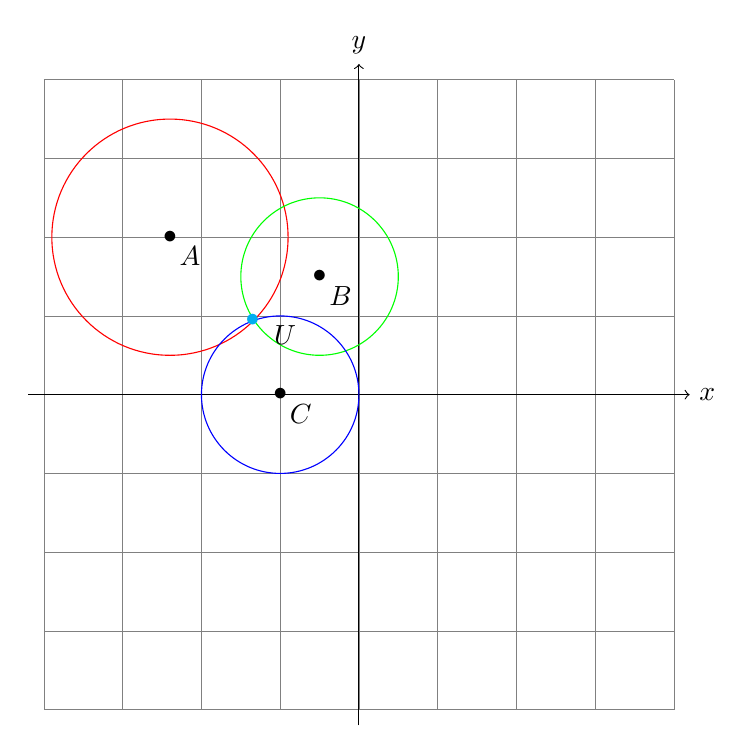
\begin{tikzpicture}
            \draw[very thin,color=gray] (-4,-4) grid (4,4);
            \draw[->] (-4.2,0) -- (4.2,0) node[right] {$x$};
            \draw[->] (0,-4.2) -- (0,4.2) node[above] {$y$};
    
            \draw[color=red] (-2.4,2) circle (1.5);
            \draw (-2.4,2) node {$\bullet$};
            \node[anchor=north west] at (-2.4,2) {$A$};
        
            \draw[color=green] (-0.5,1.5) circle (1);
            \draw (-0.5,1.5) node {$\bullet$};
            \node[anchor=north west] at (-0.5,1.5) {$B$};
        
            \draw[color=blue] (-1,0) circle (1); %2-2sqrt(3)
            \draw (-1,0) node {$\bullet$};
            \node[anchor=north west] at (-1,0) {$C$};
        
            \draw (-1.35,0.95) [cyan] node {$\bullet$};
            \node[anchor=north west] at (-1.2,1) {$U$};   
        \end{tikzpicture}
    }
    %\includegraphics{}
    \caption{Trilateration with noise $=0$}
    \label{fig:trilOK}
\end{figure}
When we step into reality however the disturbances of the signal inevitably lead to wrong estimation of the distance between the current node and the unknown node, causing the circles to intersect in wrong points or to not intersect at all, as in fig.\ref{fig:trilKO}.
\begin{figure}
    \centering
    \scalebox{1}{
        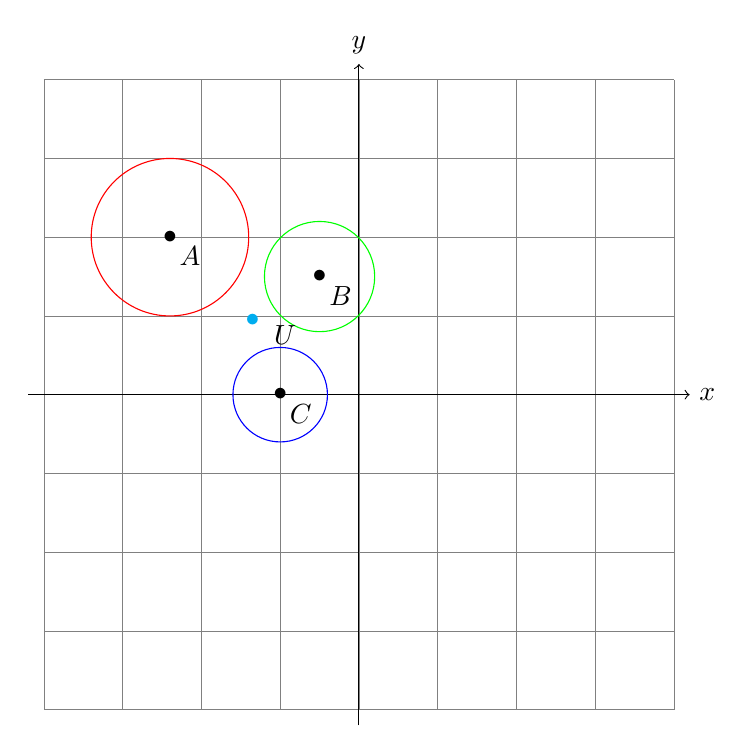
\begin{tikzpicture}
            \draw[very thin,color=gray] (-4,-4) grid (4,4);
            \draw[->] (-4.2,0) -- (4.2,0) node[right] {$x$};
            \draw[->] (0,-4.2) -- (0,4.2) node[above] {$y$};
    
            \draw[color=red] (-2.4,2) circle (1);
            \draw (-2.4,2) node {$\bullet$};
            \node[anchor=north west] at (-2.4,2) {$A$};
        
            \draw[color=green] (-0.5,1.5) circle (0.7);
            \draw (-0.5,1.5) node {$\bullet$};
            \node[anchor=north west] at (-0.5,1.5) {$B$};
        
            \draw[color=blue] (-1,0) circle (0.6); %2-2sqrt(3)
            \draw (-1,0) node {$\bullet$};
            \node[anchor=north west] at (-1,0) {$C$};
            
            \draw (-1.35,0.95) [cyan] node {$\bullet$};
            \node[anchor=north west] at (-1.2,1) {$U$};
        \end{tikzpicture}
    }
    %\includegraphics{}
    \caption{Trilateration with noise $\neq0$}
    \label{fig:trilKO}
\end{figure}
In the latter case, provided the algorithm has no software-level exception-catching, it would cause a runtime error and give no results at all. However, some improvements can be applied. The most intuitive one is to consider from the RSSI read, not just a single value but taking the max and the min values recorded during the sampling phase, and draw an annulus of possible locations as follows:
\begin{algorithm}[H]
\SetAlgoLined
\KwResult{min, max: radii of the annulus}
 Set samples = $\emptyset$\;
 \While{samples.size() < 10}{
    samples.add(new measurement)\;
 }
 min = samples.min()\;
 max = samples.max()\;
 \caption{Obtaining the derived values}
\end{algorithm}
\noindent\\The new distances will be obtained as follows:
\begin{equation}
    d_i^{min}=10^{\frac{\upsilon_0-min}{10\alpha}}    
\end{equation}
\begin{equation}
    d_i^{max}=10^{\frac{\upsilon_0-max}{10\alpha}}    
\end{equation}
The result is now given as an area that corresponds to the intersection of all the three annuli, shown in fig \ref{fig:annulus}.
\begin{figure}
    \centering
    \scalebox{1.7}{
        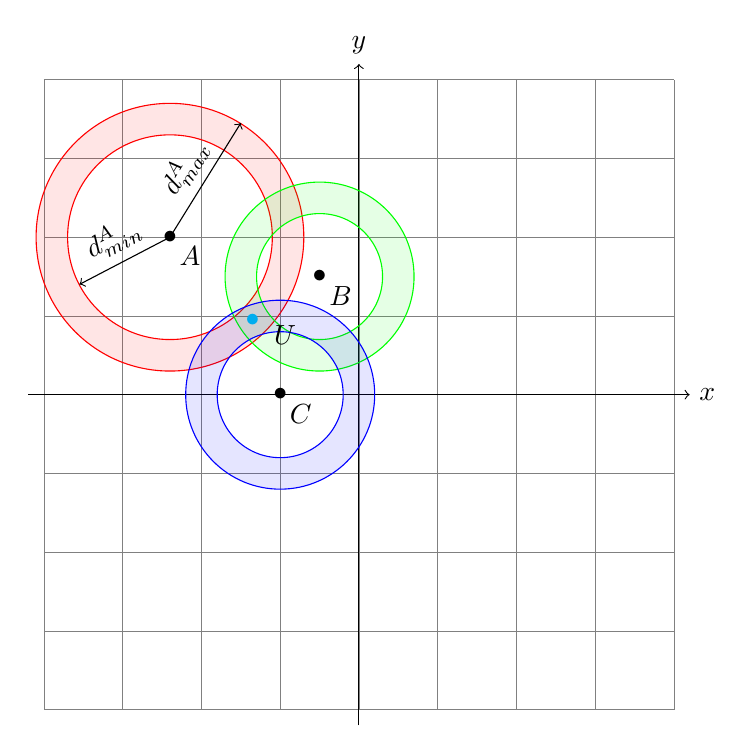
\begin{tikzpicture}
            \draw[very thin,color=gray] (-4,-4) grid (4,4);
            \draw[->] (-4.2,0) -- (4.2,0) node[right] {$x$};
            \draw[->] (0,-4.2) -- (0,4.2) node[above] {$y$};
    
            \draw[color=red] (-2.4,2) circle (1.5+0.2);
            \draw[color=red] (-2.4,2) circle (1.5-0.2);
            \fill [red,even odd rule,opacity=0.1] (-2.4,2) circle[radius=1.5+0.2] circle[radius=1.5-0.2];
            \draw[->](-2.4,2) -- (-1.5,3.45) node[midway,above,sloped] {$d^A_{max}$};
            \draw[->](-2.4,2) -- (-3.55,1.4) node[midway,above,sloped] {$d^A_{min}$};
            \draw (-2.4,2) node {$\bullet$};
            \node[anchor=north west] at (-2.4,2) {$A$};
        
            \draw[color=green] (-0.5,1.5) circle (1+0.2);
            \draw[color=green] (-0.5,1.5) circle (1-0.2);
            \fill [green,even odd rule,opacity=0.1] (-0.5,1.5) circle[radius=1+0.2] circle[radius=1-0.2];
            \draw (-0.5,1.5) node {$\bullet$};
            \node[anchor=north west] at (-0.5,1.5) {$B$};
        
            \draw[color=blue] (-1,0) circle (1+0.2); %2-2sqrt(3)
            \draw[color=blue] (-1,0) circle (1-0.2);
            \fill [blue,even odd rule,opacity=0.1] (-1,0) circle[radius=1+0.2] circle[radius=1-0.2];
            \draw (-1,0) node {$\bullet$};
            \node[anchor=north west] at (-1,0) {$C$};
            
            \draw (-1.35,0.95) [cyan] node {$\bullet$};
            \node[anchor=north west] at (-1.2,1) {$U$};
        \end{tikzpicture}
    }
    %\includegraphics{}
    \caption{Trilateration with noise compensation}
    \label{fig:annulus}
\end{figure}
Although the results are quite promising, this algorithm is rarely used, due to the computation difficulties of treating annuli. One important drawback is the low number of measurements exploited. Clearly, a higher number of samples implies a lower influence of the noise on the final estimation.
\clearpage

\section{Min Max}
\begin{center}
    \begin{tabular}{ |c|c| } 
    \hline
    \multicolumn{2}{|c|}{ \textbf{Assume to know:} } \\
    \hline
    $\upsilon_0$ & $\alpha$ \\
    \hline
    \end{tabular}
\end{center}
Consider the previous framework. As usual one can deduce the distance of the unknown node, by reverting the propagation model as done in the previous section. Then we can obtain a number of circumferences, one for each anchor node, that represent the possible locations of the unknown node. In this algorithm, however, you need to consider not circles but squares. The development of this algorithm follows \cite{inproceedings}. Each anchor node $i$ with estimated distance $d_i$ from node $u,u>n$ (with \ref{eq:18}) is associated to a square centered in $(x_i,y_i)$ with side equal to $2d_i$. At this point, one has a set of overlapping squares, and can easily find the intersection of all those squares,  which results in a rectangles of vertices $(x_{min},y_{min}), (x_{max},y_{min}), (x_{max},y_{max}), (x_{min},y_{max})$ with the following equations:
\begin{equation}
    x_{min}=\max(x_1-d_1,...,x_n-d_n)
\end{equation}
\begin{equation}
    x_{max}=\min(x_1+d_1,...,x_n+d_n)
\end{equation}
\begin{equation}
    y_{min}=\max(y_1-d_1,...,y_n-d_n)
\end{equation}
\begin{equation}
    y_{max}=\min(y_1+d_1,...,y_n+d_n)
\end{equation}
The final location will be estimated as the center of this rectangle, as follows:
\begin{equation}
    x_u=\frac{x_{min}+x_{max}}{2}
\end{equation}
\begin{equation}
    y_u=\frac{y_{min}+y_{max}}{2}
\end{equation}
The gray area in \ref{fig:mmax} shows the intersection of all the squares.
\begin{figure}
    \centering
    \scalebox{1.7}{
        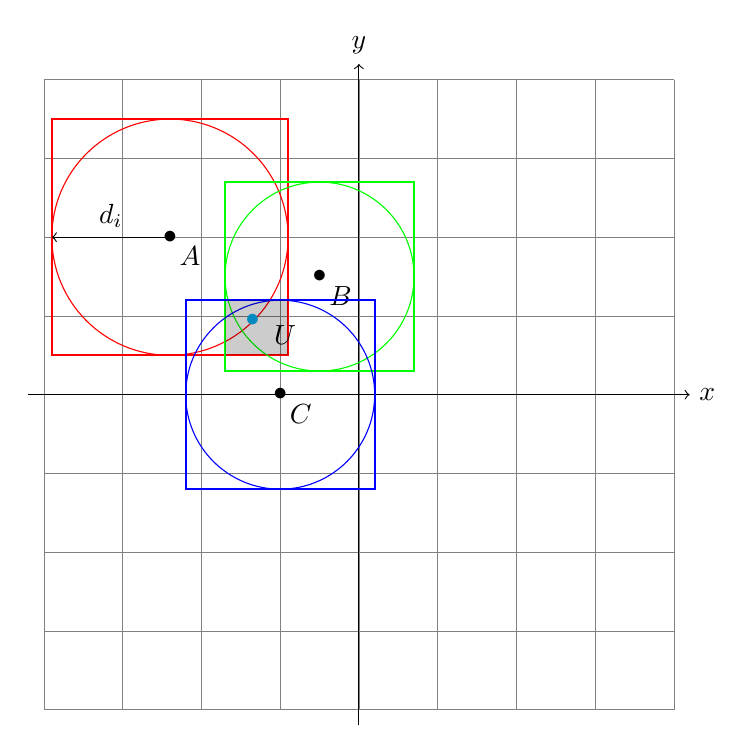
\begin{tikzpicture}
            \draw[very thin,color=gray] (-4,-4) grid (4,4);
            \draw[->] (-4.2,0) -- (4.2,0) node[right] {$x$};
            \draw[->] (0,-4.2) -- (0,4.2) node[above] {$y$};
    
            \draw[color=red] (-2.4,2) circle (1.5);
            \draw[red, thick] (-3.9,0.5) rectangle (-0.9,3.5);
            \draw[->](-2.4,2) -- (-3.9,2) node[midway,above,sloped] {$d_i$};
            \draw (-2.4,2) node {$\bullet$};
            \node[anchor=north west] at (-2.4,2) {$A$};
        
            \draw[color=green] (-0.5,1.5) circle (1.2);
            \draw[green, thick] (-1.7,0.3) rectangle (0.7,2.7);
            \draw (-0.5,1.5) node {$\bullet$};
            \node[anchor=north west] at (-0.5,1.5) {$B$};
        
            \draw[color=blue] (-1,0) circle (1.2); %2-2sqrt(3)
            \draw[blue, thick] (-2.2,-1.2) rectangle (0.2,1.2);
            \draw (-1,0) node {$\bullet$};
            \node[anchor=north west] at (-1,0) {$C$};
            
            \draw (-1.35,0.95) [cyan] node {$\bullet$};
            \node[anchor=north west] at (-1.2,1) {$U$};
            
            \fill [opacity=0.2] (-0.9,1.2) rectangle (-1.7,0.5);
        \end{tikzpicture}
    }
    %\includegraphics{}
    \caption{Min-Max estimation}
    \label{fig:mmax}
\end{figure}
\clearpage

\section{Linear estimation}
\textbf{Assume to know:} $$\upsilon_0\qquad \alpha\qquad\xi_i,\forall i$$\\
In \cite{rzk} you can find this version but using a slightly different model.
Consider the model \ref{eq:5} below reported
\begin{equation}
    \nu_i=-\beta\ln(d_i)+\xi_i
    \label{eq:15}
\end{equation}
After some time, for each anchor node, we will have a list of measurements, drawn from the random variable 
\begin{equation}
-\beta\ln(d_i)+\xi_i\sim \mathcal{N}(-\beta\ln(d_i),\sigma_i^2)
\label{eq:14}
\end{equation}
Rewrite the \ref{eq:15} as follows 
\begin{equation}
    \nu_i=-\ln\big(d_i^{2\frac{\beta}{2}}\big)+\xi_i
    \label{eq:6}
\end{equation}
By exponentiating both members of \ref{eq:6} we have 
\begin{equation}
    e^{\nu_i}=e^{-\ln\big(d_i^{2\frac{\beta}{2}}\big)+\xi_i}
\end{equation}
\begin{equation}
    \bigg(e^{\nu_i}\bigg)^{-1}=\bigg(e^{-\ln\big(d_i^{2\frac{\beta}{2}}\big)+\xi_i}\bigg)^{-1}
\end{equation}
\begin{equation}
    e^{-\nu_i}=e^{\ln\big(d_i^{2\frac{\beta}{2}}\big)-\xi_i}
\end{equation}
\begin{equation}
    e^{-\nu_i}=d_i^{2\frac{\beta}{2}}e^{-\xi_i}
\end{equation}
\begin{equation}
    \bigg(e^{-\nu_i}\bigg)^{\frac{2}{\beta}}=\bigg(d_i^{2\frac{\beta}{2}}e^{-\xi_i}\bigg)^{\frac{2}{\beta}}
\end{equation}
\begin{equation}
    e^{-\frac{2}{\beta}\nu_i}=d_i^2e^{-\frac{2}{\beta}\xi_i}
\end{equation}
Remind that the exponentiation of a gaussian distribution is \cite{Beran2011} a log-normal distribution. In other words, given $X\sim \mathcal{N}(\mu,\sigma^2)$, then $Y=e^X\sim \text{Lognormal}(\mu,\sigma^2)$ with
\begin{equation}
    E[Y]=E\big[e^X\big]=e^{\mu+\frac{\sigma^2}{2}}
    \label{eq:20}
\end{equation}
\begin{equation}
    Var[Y]=Var\big[e^X\big]=(e^{\sigma^2}-1)e^{2\mu+\sigma^2}
    \label{eq:7}
\end{equation}
From \cite{alma9926534668905776}, it is clear also that if $a\in \mathbb{R}$ and $X\sim \mathcal{N}(\mu,\sigma^2)$ then
\begin{equation}
aX\sim \mathcal{N}(a\mu,a^2\sigma^2)    
\end{equation}
so in this case, 
\begin{equation}
    -\frac{2}{\beta}\xi_i\sim \mathcal{N}\bigg(0,\frac{4}{\beta^2}\sigma^2_i\bigg)
\end{equation}
From equations \ref{eq:20} and \ref{eq:7}
\begin{align}
    &E\bigg[e^{-\frac{2}{\beta}\nu_i}\bigg]\\
    &=E\bigg[d_i^2e^{-\frac{2}{\beta}\xi_i}\bigg]\\
    &=d_i^2E\bigg[e^{-\frac{2}{\beta}\xi_i}\bigg]\\ &=d_i^2e^{\frac{2}{\beta^2}\sigma^2_i}
    \label{eq:8}
\end{align}
\begin{align}
    &Var\bigg[e^{-\frac{2}{\beta}\nu_i}\bigg]\\
    &=Var\bigg[d_i^2e^{-\frac{2}{\beta}\xi_i}\bigg]\\
    &=d_i^4Var\bigg[e^{-\frac{2}{\beta}\xi_i}\bigg]\\
    &=d_i^4(e^{\frac{4}{\beta^2}\sigma_i^2}-1)e^{\frac{4}{\beta^2}\sigma^2_i}
    \label{eq:21}
\end{align}
As we can see from \ref{eq:8}, $e^{-\frac{2}{\beta}\nu_i}$ is a biased estimate of $d_i^2$, however we can remove its bias by dividing it by $e^{\frac{2}{\beta^2}\sigma^2_i}$ (which is the bias itself). Therefore, an unbiased estimate of $d_i^2$ is 
\begin{equation}
    \hat{d}_i^2=e^{-\frac{2}{\beta}\nu_i-\frac{2}{\beta^2}\sigma^2_i}
    \label{eq:9}
\end{equation}
We want to use the above estimator obtained from the measurements to build a linear model in $\mathbf{x}$. Since the estimator is now unbiased by writing 
\begin{equation}
    (x_u-x_i)^2+(y_u-y_i)^2=\hat{d}_i^2
\end{equation}
we can write
\begin{equation}
    (x_u-x_i)^2+(y_u-y_i)^2=e^{-\frac{2}{\beta}\nu_i-\frac{2}{\beta^2}\sigma^2_i}
\end{equation}
\begin{equation}
    -2x_ix_u-2y_iy_u+x^2_u+y^2_u+x_i^2+y_i^2=e^{-\frac{2}{\beta}\nu_i-\frac{2}{\beta^2}\sigma^2_i}
\end{equation}
\begin{equation}
    -2x_ix_u-2y_iy_u+x_u^2+y_u^2=e^{-\frac{2}{\beta}\nu_i-\frac{2}{\beta^2}\sigma^2_i}-x_i^2-y_i^2
\end{equation}
By setting the condition 
\begin{equation}
R^2=x_u^2+y_u^2    
\label{eq:10}
\end{equation}
we can write it in matrix form
\begin{equation}
    \begin{bmatrix}
        -2x_1 & -2y_1 & 1\\
        \vdots&\vdots&\vdots\\
        -2x_n & -2y_n & 1
    \end{bmatrix}
    \begin{bmatrix}
        x_u\\
        y_u\\
        R^2
    \end{bmatrix} = 
    \begin{bmatrix}
       e^{-\frac{2}{\beta}\nu_1-\frac{2}{\beta^2}\sigma^2_1} & -x_1^2 & -y_1^2\\
        \vdots&\vdots&\vdots\\
        e^{-\frac{2}{\beta}\nu_n-\frac{2}{\beta^2}\sigma^2_n} & -x_n^2 & -y_n^2\\
    \end{bmatrix}
\end{equation}
with $$\mathbf{A}=\begin{bmatrix}
        -2x_1 & -2y_1 & 1\\
        \vdots&\vdots&\vdots\\
        -2x_n & -2y_n & 1
    \end{bmatrix}$$
$$\mathbf{x} =     \begin{bmatrix}
        x_u\\
        y_u\\
        R^2
    \end{bmatrix}$$
$$\mathbf{b}=    \begin{bmatrix}
        e^{-\frac{2}{\beta}\nu_1-\frac{2}{\beta^2}\sigma^2_1} & -x_1^2 & -y_1^2\\
        \vdots&\vdots&\vdots\\
        e^{-\frac{2}{\beta}\nu_n-\frac{2}{\beta^2}\sigma^2_n} & -x_n^2 & -y_n^2\\
    \end{bmatrix}$$
Now since $\mathbf{x^*}$ is unknown we would like to choose $\mathbf{x}\approx\mathbf{x^*}$ to have 
\begin{equation}
    \mathbf{Ax-b}\approx0
\end{equation}
One easy way is to seek the minimum of 
\begin{align}
    J(\mathbf{x})&=\mathbf{(Ax-b)^T(Ax - b)}\\
    &=\mathbf{x^TA^TAx-2x^TA^Tb+b^Tb}
\end{align}
We can fit this model with the Least Square Method, that for a linear model (which is ours) has a known explicit solution \cite{10.5555/1557273} that can be easily verified. In fact since $J(\mathbf{x})$ is a quadratic function of $\mathbf{x}$, then there is a unique minimum \cite{Ortega1987,rzk}. The LLS estimate corresponds to:
\begin{equation}
    \hat{\mathbf{x}}=\arg \min_\mathbf{x} J(\mathbf{x})
\end{equation}
which can be found by setting to $0$ its derivative
    
\begin{align}
\begin{split}
&\frac{\partial J(\mathbf{x})}{\partial \mathbf{x}}=0\\
    &2\mathbf{A^TA}\hat{\mathbf{x}}-2\mathbf{A^Tb}=0\\
    &\mathbf{A^TA\hat{x}}=\mathbf{A^Tb}\\
    &\hat{\mathbf{x}}=\mathbf{(A^TA)^{-1}A^Tb}
\end{split}
\end{align}
The target position can be finally obtained as 
\begin{equation}
\begin{bmatrix}
    \hat{x}_u\\
    \hat{y}_u
\end{bmatrix}=
\begin{bmatrix}
    [\hat{\mathbf{x}}]_1\\
    [\hat{\mathbf{x}}]_2
\end{bmatrix}
\end{equation}
\clearpage


\section{Weighted linear estimation}
\begin{center}
    \begin{tabular}{ |c|c|c| } 
    \hline
    \multicolumn{3}{|c|}{ \textbf{Assume to know:} } \\
    \hline
    $\upsilon_0$ & $\alpha$ & $\xi_i,\forall i$\\
    \hline
    \end{tabular}
\end{center}    
In the previous section we have seen how to use statistics to obtain an estimator of the distance from each anchor node to the unknown node, and then putting all this in a linear form, to deduce the location of the unknown node with a simple closed formula such as the linear least squares. However we can still improve it by givin to each anchor node a weight, bound to the variance of the estimator $\hat{d}_i^2$ obtained from the anchor node $i$. A good idea would be to give more importance to the nodes that produces an estimator with low variance, and to give less importance to those node that produces estimators with high variance. To ease the computation we consider each anchor node to be indepentendet from each other. One way to do that is to introduce a symmetric covariance matrix $\mathbf{W}'$, which is also diagonal (because of the independence of anchor nodes). Since we want the weight assigned to each node to be inversely proportional to the variance we consider $\mathbf{W}=(\mathbf{W}')^{-1}$ \cite{rzk,899498y4hd}. It is important to note that this improvement does not regard the generation of the vector of estimators, rather the minimization of the cost function. Now we compute the variance of the estimator $\hat{d}_i^2$
\begin{align}
\sigma^2_{\hat{d_i}}=&Var\big[\hat{d_i^2}\big]=&& \\
&=Var\bigg[e^{-\frac{2}{\beta}\nu_i-\frac{2}{\beta^2}\sigma^2_i}\bigg] && \text{from \ref{eq:9}}\\
&=\bigg(e^{-\frac{2}{\beta^2}\sigma^2_i}\bigg)^2Var\bigg[e^{-\frac{2}{\beta}\nu_i}\bigg]&& \text{because it is a constant}\\
&=\cancel{e^{-\frac{4}{\beta^2}\sigma^2_i}}d_i^4\bigg(e^{\frac{4}{\beta^2}\sigma_i^2}-1\bigg)\cancel{e^{\frac{4}{\beta^2}\sigma^2}} &&\text{from } \ref{eq:21}\\
&=d_i^4\bigg(e^{\frac{4}{\beta^2}\sigma_i^2}-1\bigg)\\
&\approx \big(\hat{d_i}^2\big)^2\bigg(e^{\frac{4}{\beta^2}\sigma_i^2}-1\bigg)\\
&=\bigg(e^{-\frac{2}{\beta}\nu_i-\frac{2}{\beta^2}\sigma^2_i}\bigg)^2\bigg(e^{\frac{4}{\beta^2}\sigma_i^2}-1\bigg)&&\text{from }\ref{eq:9}\\
&=e^{-\frac{4}{\beta}\nu_i-\frac{4}{\beta^2}\sigma^2_i}\bigg(e^{\frac{4}{\beta^2}\sigma^2_i}-1\bigg)\\
&=e^{-\frac{4}{\beta}\nu_i}\bigg(1-e^{-\frac{4}{\beta^2}\sigma^2_i}\bigg)\\
&=\frac{1-e^{-\frac{4}{\beta^2}\sigma^2_i}}{e^{\frac{4}{\beta}\nu_i}}
\end{align}
The covariance matrix of the estimators is $$\mathbf{W}'=\text{diag}\big(\sigma^2_{\hat{d_1}},...,\sigma^2_{\hat{d_n}}\big)$$
Now we get to the weighting matrix
\begin{align}
    \mathbf{W}&=\big(\mathbf{W'}\big)^{-1}=\text{diag}\big((\sigma^2_{\hat{d_1}})^{-1},...,(\sigma^2_{\hat{d_n}})^{-1}\big)\\
    &=\text{diag}\bigg(\frac{e^{\frac{4}{\beta}\nu_1}}{1-e^{-\frac{4}{\beta^2}\sigma^2_1}},...,\frac{e^{\frac{4}{\beta}\nu_n}}{1-e^{-\frac{4}{\beta^2}\sigma^2_n}}\bigg)
\end{align}
The improved cost function \cite{rzk} takes the following form 
\begin{align}
    J&(\mathbf{x})=\mathbf{(Ax-b)^TW(Ax - b)}\\
    &=\mathbf{x^TA^TWAx-2x^TA^TWb+b^TWb}
\end{align}
that can be minimized with the usual LLS
\begin{align}
    \mathbf{\hat{x}=(A^TWA)^{-1}A^TWb}
\end{align}
The precision of this estimation can be further improved by imposing the constraint \ref{eq:10} on the minimization. This condition is ignored if we use LLS, but it can be successfully employed with the method of Lagrange multipliers \cite{1275684,Lopez1994, pasa}.


\clearpage

\section{Quadratic linearization}
  \begin{center}
  \textbf{Assume to know:}
  \begin{itemize}
    \centering
    \item $\upsilon_0$
    \item $\alpha$
  \end{itemize}
  \end{center}
From the canonical model extract $d_i$ as follows
\begin{equation*}
    10^{\upsilon_{i}}=10^{\upsilon_0-10\alpha\log_{10}(d_i)}
\end{equation*}
\begin{equation*}
    10^{\upsilon_{i}-\upsilon_0}=10^{-10\alpha\log_{10}(d_i)}
\end{equation*}
\begin{equation*}
     10^{\upsilon_{i}-\upsilon_0}=d_i^{-10\alpha}
\end{equation*}
\begin{equation}
    d_i=10^{\frac{\upsilon_0-\upsilon_{i}}{10\alpha}}
    \label{eq:17}
\end{equation}
so that we have the following set of equations
\begin{align}
\begin{split} 
(x_1-x)^2+(y_1-y)^2&=d_1^2 \\ 
(x_2-x)^2+(y_2-y)^2&=d_2^2 \\ 
&\;\;\vdots\\
(x_n-x)^2+(y_n-y)^2&=d_n^2 \\
\end{split}
\label{eq:11}
\end{align}
Consider 
\begin{align}
\frac{1}{n}&\sum_{i=1}^nd_i^2=\\
&=\frac{1}{n}\sum_{i=1}^n\big[(x_i-x)^2+(y_i-y)^2\big]\\
&=\frac{1}{n}\sum_{i=1}^n(x_i-x)^2+\frac{1}{n}\sum_{i=1}^n(y_i-y)^2\\
&=\frac{1}{n}\sum_{i=1}^n[x_i^2-2x_ix+x^2] + \frac{1}{n}\sum_{i=1}^n[y_i^2-2y_iy+y^2]\\
&=\frac{1}{n}\sum_{i=1}^n[x_i^2]-2x\frac{1}{n}\sum_{i=1}^n[x_i]+ x^2 + \frac{1}{n}\sum_{i=1}^n[y_i^2]-2y\frac{1}{n}\sum_{i=1}^n[y_i]+ y^2
\end{align}
which is finally
\begin{equation}
    \frac{1}{n}\sum_{i=1}^n[x_i^2]-2x\frac{1}{n}\sum_{i=1}^n[x_i]+ x^2 + \frac{1}{n}\sum_{i=1}^n[y_i^2]-2y\frac{1}{n}\sum_{i=1}^n[y_i]+ y^2= \frac{1}{n}\sum_{i=1}^nd_i^2
    \label{eq:12}
\end{equation}
Frone one of the \ref{eq:11} it follows
\begin{align}
x_i^2+x^2-2x_ix+y_i^2+y^2-2y_iy&=d_i^2 &&\text{develop the square}\\ 
-x_i^2-x^2+2x_ix-y_i^2-y^2+2y_iy&=-d_i^2 && \text{multiply by } -1
\label{eq:13}
\end{align}
Now by adding member to member \ref{eq:12} to \ref{eq:13} you have 
\begin{equation}
\begin{split}
    \bigg(-x_i^2  + \frac{1}{n}\sum_{i=1}^n[x_i^2]\bigg)+
    \bigg(-y_i^2+ \frac{1}{n}\sum_{i=1}^n[y_i^2]\bigg)+\\
    +\bigg(2x_ix-2x\frac{1}{n}\sum_{i=1}^n[x_i]\bigg)+
    \bigg(2y_iy -2y\frac{1}{n}\sum_{i=1}^n[y_i]\bigg)
    =\frac{1}{n}&\sum_{i=1}^n[d_i^2]-d_i^2
\end{split}    
\end{equation}
and by rearranging the equation
\begin{equation}
\begin{split}
    +2x\bigg(x_i-\frac{1}{n}\sum_{i=1}^n[x_i]\bigg)+
    2y\bigg(y_i -\frac{1}{n}\sum_{i=1}^n[y_i]\bigg)+\\
    +\bigg(-x_i^2  + \frac{1}{n}\sum_{i=1}^n[x_i^2]\bigg)+
    \bigg(-y_i^2+ \frac{1}{n}\sum_{i=1}^n[y_i^2]\bigg)
    =\frac{1}{n}&\sum_{i=1}^n[d_i^2]-d_i^2
\end{split}    
\end{equation}
Then the previous set of equations \ref{eq:11} becomes
\begin{align}
\begin{split} 
    \bigg(x_1-\frac{1}{n}&\sum_{i=1}^nx_i\bigg)x+\bigg(y_1-\frac{1}{n}\sum_{i=1}^ny_i\bigg)y\\
    &=\frac{1}{2}\bigg[\bigg(x_1^2-\frac{1}{n}\sum_{i=1}^nx^2_i\bigg)+\bigg(y_1^2-\frac{1}{n}\sum_{i=1}^ny^2_i\bigg)-\bigg(d_1^2-\frac{1}{n}\sum_{i=1}^nd_i^2\bigg)\bigg]\\
&\;\;\vdots\\
    \bigg(x_n-\frac{1}{n}&\sum_{i=1}^nx_i\bigg)x+\bigg(y_n-\frac{1}{n}\sum_{i=1}^ny_i\bigg)y\\
    &=\frac{1}{2}\bigg[\bigg(x_n^2-\frac{1}{n}\sum_{i=1}^nx^2_i\bigg)+\bigg(y_n^2-\frac{1}{n}\sum_{i=1}^ny^2_i\bigg)-\bigg(d_n^2-\frac{1}{n}\sum_{i=1}^nd_i^2\bigg)\bigg]
\end{split}
\end{align}
So can write the above set of equations in matrix form $\mathbf{Ax}=\mathbf{b}$ by setting
$$
\mathbf{A}=\begin{bmatrix}
    x_1-\frac{1}{n}\sum_{i=1}^nx_i&y_1-\frac{1}{n}\sum_{i=1}^ny_i\\
    \vdots&\vdots\\
    x_n-\frac{1}{n}\sum_{i=1}^nx_i&y_n-\frac{1}{n}\sum_{i=1}^ny_i
\end{bmatrix}
$$
$$
\mathbf{x}=\begin{bmatrix}
    x\\
    y
\end{bmatrix}
$$
$$\mathbf{b}=\frac{1}{2}
\begin{bmatrix}
\bigg(x_1^2-\frac{1}{n}\sum_{i=1}^nx^2_i\bigg)+\bigg(y_i^2-\frac{1}{n}\sum_{i=1}^ny^2_i\bigg)-\bigg(d_i^2-\frac{1}{n}\sum_{i=1}^nd_i^2\bigg)\\
\vdots\\
\bigg(x_n^2-\frac{1}{n}\sum_{i=1}^nx^2_i\bigg)+\bigg(y_n^2-\frac{1}{n}\sum_{i=1}^ny^2_i\bigg)-\bigg(d_n^2-\frac{1}{n}\sum_{i=1}^nd_i^2\bigg)
\end{bmatrix}
$$
Both $\mathbf{A}$ and $\mathbf{b}$ are completely known, also $d_i$, due to \ref{eq:17}. Then the solution can be computed with the usual Linear Least Square procedure obtaining
\begin{equation}
    \mathbf{x}=(\mathbf{A^TA})^{-1}\mathbf{A^Tb}
\end{equation}
\clearpage


\section{Lines intersection}
  \begin{center}
  \textbf{Assume to know:}
  \begin{itemize}
    \centering
    \item $\upsilon_0$
    \item $\alpha$
  \end{itemize}
  \end{center}
Let's start from a geometrical analysis. Given two intersecting circles at center $x_{1},y_{1}$ and $x_{2},y_{2}$ respectively and with radius $r_1$ and $r_2$ respectively, the line that passes by the two points of intersection has the following equation \cite{rzk}
\begin{equation}
    (x_2-x_1)x+(y_2-y_1)y=\frac{1}{2}\big[(x_2^2+y_2^2)-(x_1^2+y_1^2)-(r_2^2-r_1^2)\big]
    \label{eq:25}
\end{equation}
or equivalently
\begin{equation}
    y=\frac{1}{y_2-y_1}\bigg(-(x_2-x_1)x+\frac{1}{2}\big(x_2^2+y_2^2-r_2^2-(x_1^2+y_1^2-r_1^2)\big)\bigg)
\end{equation}
Note that the formula is still valid even if the two circles do not intersect each other.
Given $n$ measurements (so $n$ circles), only $n-1$ lines are needed to have an independent system of equations. For example, suppose to have three circles, it is needed to have only 2 lines, for example the line passing between the first and the second circle, and the line passing between the first and the third one, as in fig \ref{fig:1}.
Therefore, given $n$ points we have a set of $n-1$ equations like the above \ref{eq:25}, that can be written in matrix form $\mathbf{Ax}=\mathbf{b}$ with
$$\mathbf{A}=\begin{bmatrix}
x_2-x_1&y_2-y_1\\
x_3-x_1&y_3-y_1\\
\vdots&\vdots\\
x_n-x_1&y_n-y_1
\end{bmatrix}$$
$$\mathbf{x}=\begin{bmatrix}
x\\
y
\end{bmatrix}$$
$$\mathbf{b}=\frac{1}{2}\begin{bmatrix}
(x^2_2+y^2_2)-(x_1^2+y^2_1)-(d_2^2-d_1^2)\\
(x^2_3+y^2_3)-(x_1^2+y^2_1)-(d_3^2-d_1^2)\\
\vdots\\
(x^2_n+y^2_n)-(x_1^2+y^2_1)-(d_n^2-d_1^2)\\
\end{bmatrix}$$
where the $d_i$ are computed with the \ref{eq:17}.\\\\
The solution is obtained as an approximated intersection of all these lines with the LLS, as in fig. \ref{fig:2}. You can see that they do not need to intersect in exactly one point, that's why the solution is computed using LLS. In cyan it is shown the real position of the unknown node (U).
\begin{figure}
    \centering
    \scalebox{1.2}{
        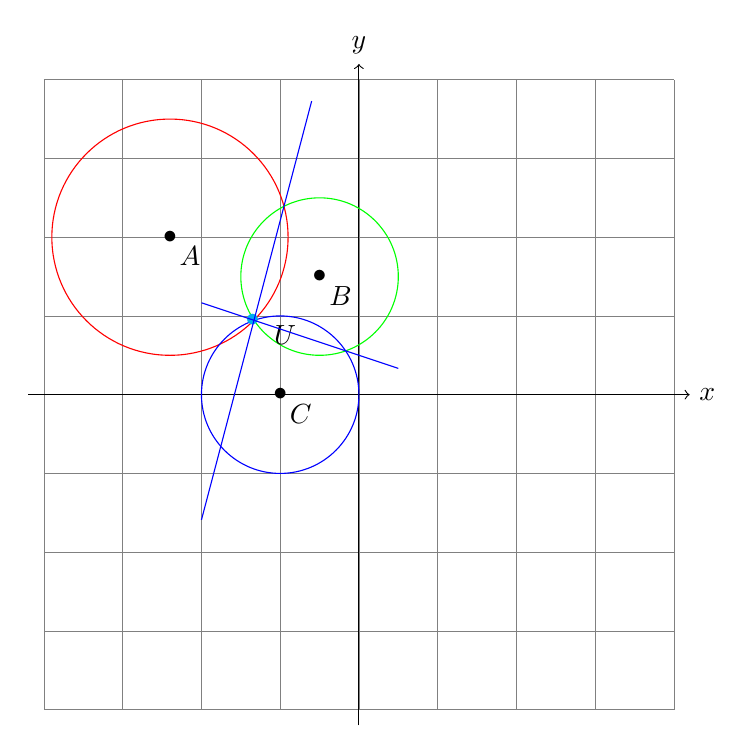
\begin{tikzpicture}
            \draw[very thin,color=gray] (-4,-4) grid (4,4);
            \draw[->] (-4.2,0) -- (4.2,0) node[right] {$x$};
            \draw[->] (0,-4.2) -- (0,4.2) node[above] {$y$};
    
            \draw[color=red] (-2.4,2) circle (1.5);
            \draw (-2.4,2) node {$\bullet$};
            \node[anchor=north west] at (-2.4,2) {$A$};
        
            \draw[color=green] (-0.5,1.5) circle (1);
            \draw (-0.5,1.5) node {$\bullet$};
            \node[anchor=north west] at (-0.5,1.5) {$B$};
        
            \draw[color=blue] (-1,0) circle (1); %2sqrt(3)
            \draw (-1,0) node {$\bullet$};
            \node[anchor=north west] at (-1,0) {$C$};
            
            \draw (-1.35,0.95) [cyan] node {$\bullet$};
            \node[anchor=north west] at (-1.2,1) {$U$};
            
            \draw[scale=1, domain=-2:-0.6, smooth, variable=\x, blue] plot ({\x}, {-((+2.4-0.5)/(1.5-2))*\x
            +1/(2*(1.5-2))*(0.5^2+1.5^2-1-(2.4^2+2^2-1.5^2))});
            
            \draw[scale=1, domain=-2:0.5, smooth, variable=\x, blue] plot ({\x}, {(1/(-1.5))*(-(-1+0.5)*\x+0.5*(1-1-(0.5^2+1.5^2-1)))});
            
            %\draw[scale=0.5, domain=-3:3, smooth, variable=\y, red]  plot ({\y*\y}, {\y});
        \end{tikzpicture}
    }
    %\includegraphics{}
    \caption{Application of the algorithm with 3 circles and 2 lines}
    \label{fig:1}
\end{figure}
\begin{figure}
    \centering
    \scalebox{1.8}{
        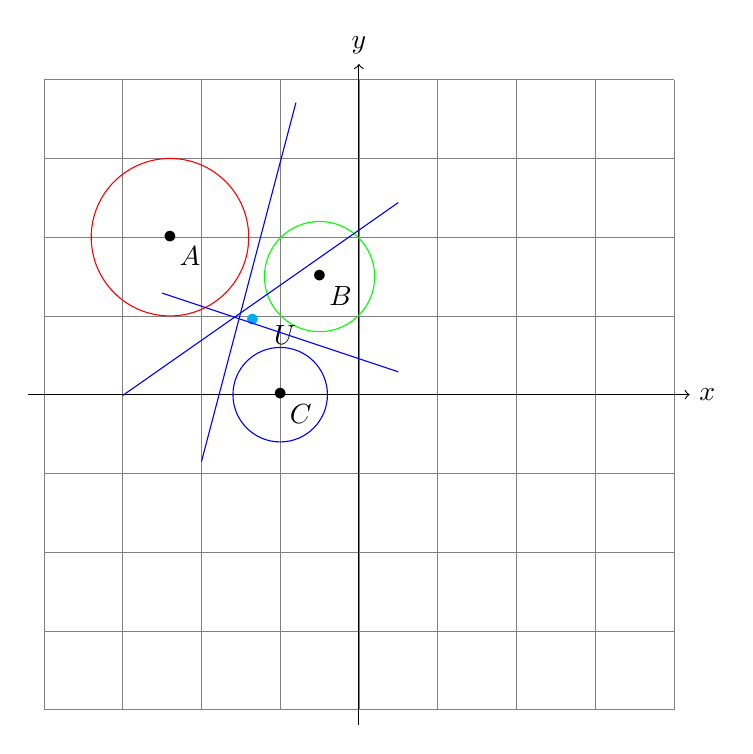
\begin{tikzpicture}
            \draw[very thin,color=gray] (-4,-4) grid (4,4);
            \draw[->] (-4.2,0) -- (4.2,0) node[right] {$x$};
            \draw[->] (0,-4.2) -- (0,4.2) node[above] {$y$};
    
            \draw[color=red] (-2.4,2) circle (1);
            \draw (-2.4,2) node {$\bullet$};
            \node[anchor=north west] at (-2.4,2) {$A$};
        
            \draw[color=green] (-0.5,1.5) circle (0.7);
            \draw (-0.5,1.5) node {$\bullet$};
            \node[anchor=north west] at (-0.5,1.5) {$B$};
        
            \draw[color=blue] (-1,0) circle (0.6); %2-2sqrt(3)
            \draw (-1,0) node {$\bullet$};
            \node[anchor=north west] at (-1,0) {$C$};
            
            \draw (-1.35,0.95) [cyan] node {$\bullet$};
            \node[anchor=north west] at (-1.2,1) {$U$};
            
            
            \draw[scale=1, domain=-2:-0.8, smooth, variable=\x, blue] plot ({\x}, {-((+2.4-0.5)/(1.5-2))*\x
            +1/(2*(1.5-2))*(0.5^2+1.5^2-0.7^2-(2.4^2+2^2-1^2))});
            
            \draw[scale=1, domain=-2.5:0.5, smooth, variable=\x, blue] plot ({\x}, {(1/(-1.5))*(-(-1+0.5)*\x+0.5*(1-0.6^2-(0.5^2+1.5^2-0.7^2)))});
            
            
            \draw[scale=1, domain=-3:0.5, smooth, variable=\x, blue] plot ({\x}, {(1/(-2))*(-(-1+2.4)*\x+0.5*(1-0.6
            -(2.4^2+2^2-1^2)))});
            
        \end{tikzpicture}
    }
    %\includegraphics{}
    \caption{Application of the algorithm with noise compensation}
    \label{fig:2}
\end{figure}
\\\\Given the high influence in this formula of the first anchor node (present in all equations), one can try an optimization by rearranging the above formula in a way that it relays more evenly to all the nodes as follows
$$\mathbf{A}=\begin{bmatrix}
x_2-x_1&y_2-y_1\\
x_3-x_2&y_3-y_2\\
\vdots&\vdots\\
x_n-x_{n-1}&y_n-y_{n-1}
\end{bmatrix}$$
$$\mathbf{x}=\begin{bmatrix}
x\\
y
\end{bmatrix}$$
$$\mathbf{b}=\frac{1}{2}\begin{bmatrix}
(x^2_2+y^2_2)-(x_1^2+y^2_1)-(d_2^2-d_1^2)\\
(x^2_3+y^2_3)-(x_2^2+y^2_2)-(d_3^2-d_2^2)\\
\vdots\\
(x^2_n+y^2_n)-(x_{n-1}^2+y^2_{n-1})-(d_n^2-d_{n-1}^2)\\
\end{bmatrix}$$
\clearpage


\section{Multilateration}
  \begin{center}
  \textbf{Assume to know:}
  \begin{itemize}
    \centering
    \item $\emptyset$
  \end{itemize}
  \end{center}
This algorithm is the generalization of the trilateration method and is known as Multilateration. 
This method can provide two main benefits over the classic trilateration:
\begin{itemize}
    \item Always exists a solution (the algorithm may not be able to find it though)
    \item The result is made on more observation than the trilateration
\end{itemize}
So, from the measurement of each node, we try straight away to fit those data to the canonical model. To do so we write a cost function to be minimized
\begin{multline}
    J(\upsilon_0,\alpha,x_u,y_u)=\\=\sum_{i=1}^n\bigg(\upsilon_i-\upsilon_0+10\alpha\log_{10}\big(\sqrt{(x_i-x_u)^2+(y_i-y_u)^2}\big)\bigg)^2
    \label{eq:23}
\end{multline}
\begin{equation}
\hat{x}_u, \hat{y}_u=\arg \min_{\upsilon_0,\alpha,x_u,y_u}J(\upsilon_0,\alpha,x_u,y_u)
\end{equation}
The great advantage of this method is that it theoretically doesn't need to know any parameter of the model, however in reality to have good results at least $\upsilon_0$ must be known. This is usually not a problem, since the signal intensity at a fixed distance can be obtained by manual measurement beforehand.\\\\
To increase the accuracy of this method, one can also redefine the cost function as
\begin{multline}
    J(\upsilon_0,\alpha_1,...,\alpha_n,x_u,y_u)=\\=\sum_{i=1}^n\bigg(\upsilon_i-\upsilon_0+10\alpha_i\log_{10}\big(\sqrt{(x_i-x_u)^2+(y_i-y_u)^2}\big)\bigg)^2
    \label{eq:22}
\end{multline}
One big drawback of this method is that convergence is not guaranteed, and it often depends from the starting guess. A ``necessary condition" for convergence is that the starting guess must be quite close to the real location of the unknown device. For this reason, the usual choice for the initial guess is the estimation obtained by the linear methods.\\\\ 
The \ref{eq:23} and \ref{eq:22} are not linear systems, therefore the solution must be computed with some iterative methods, (GN, steepest descent...) \cite{chong2013introduction}.
\clearpage


\section{Maximum Likelihood method}
  \begin{center}
  \textbf{Assume to know:}
  \begin{itemize}
    \centering
    \item $\upsilon_0$
    \item $\xi_i,\forall i$
  \end{itemize}
  \end{center}
We can start by considering the model \ref{eq:15} and \ref{eq:14}.
A look more closely related to the probability point of view is (with $p(\bullet)$ the probability density function)
\begin{equation}
    p(\nu_i)=\frac{1}{\sqrt{2\pi\sigma^2_i}}e^{-\frac{1}{2}\frac{(\nu_i+\beta\ln(d_i))^2}{\sigma^2_i}}
\end{equation}
The joint probability distribution of all the nodes (assuming independence between the nodes) \begin{equation}
    p(\nu_1,...,\nu_n)=p(\nu_1)\cdot...\cdot p(\nu_n)=\frac{1}{(2\pi)^{\frac{n}{2}}\Pi_{i=1}^n\sigma_i}e^{-\frac{1}{2}\sum_{i=1}^n\frac{(\nu_i+\beta\ln(d_i))^2}{\sigma^2_i}}
\end{equation}
And in matrix form \cite{rzk}, we can write the covariance matrix as 
\begin{equation}
    \boldsymbol{\Sigma}=\begin{bmatrix}
    \sigma^2_1 & 0 & 0\\
    0 &\ddots& 0\\
    0&0&\sigma^2_n
    \end{bmatrix}
\end{equation}
with
\begin{equation}
    \mathbf{x}=\begin{bmatrix}
    x_u\\
    y_u
    \end{bmatrix}
\end{equation}
\begin{equation}
    \mathbf{f}(\mathbf{x})=-\beta\begin{bmatrix}
\ln(\sqrt{(x_u-x_1)^2+(y_u-y_1)^2})\\
\vdots\\
\ln(\sqrt{(x_u-x_n)^2+(y_u-y_n)^2})
\end{bmatrix}
\end{equation}
To obtain
\begin{equation}
    p(\boldsymbol{\nu})=\frac{1}{(2\pi)^{\frac{n}{2}}|\boldsymbol{\Sigma}|^{\frac{1}{2}}}e^{-\frac{1}{2}\big(\boldsymbol{\nu}-\mathbf{f}(\mathbf{x})\big)\boldsymbol{\Sigma}^{-1}\big(\boldsymbol{\nu}-\mathbf{f}(\mathbf{x})\big)}
    \label{eq:16}
\end{equation}
with 
\begin{equation}
    \boldsymbol{\nu}=\begin{bmatrix}
    \nu_1\\
    \vdots\\
    \nu_n
    \end{bmatrix}
\end{equation}
For the Maximum Likelihood method we need to find the maximum of \ref{eq:16} w.r.t $\mathbf{x}$. As usual to ease the computation we consider the log. 
\begin{equation}
    \ell_n(\mathbf{x})=-\ln\big((2\pi)^{\frac{n}{2}}|\boldsymbol{\Sigma}|^{\frac{1}{2}}\big)-\frac{1}{2}\big(\boldsymbol{\nu}-\mathbf{f}(\mathbf{x})\big)^\mathbf{T}\boldsymbol{\Sigma}^{-1}\big(\boldsymbol{\nu}-\mathbf{f}(\mathbf{x})\big)
\end{equation}
The first part is independent of $\mathbf{x}$, so we need only to find the stationary point of the second part, that is 
\begin{equation}
\hat{\mathbf{x}}=\arg \min_{\beta,\mathbf{x}}\frac{1}{2}\big(\boldsymbol{\nu}-\mathbf{f}(\mathbf{x})\big)^\mathbf{T}\boldsymbol{\Sigma}^{-1}\big(\boldsymbol{\nu}-\mathbf{f}(\mathbf{x})\big)
\end{equation}
As the Multilateration case, the minimization must be done with iterative algorithms.

\clearpage
\section{Centroid algorithm}
  \begin{center}
  \textbf{Assume to know:}
  \begin{itemize}
    \centering
    \item $\emptyset$
  \end{itemize}
  \end{center}
\begin{algorithm}[H]
\SetAlgoLined
\KwResult{Estimated position of the unknown node}
 Each node $i$ broadcasts its position $(x_i,y_i)$ to every other node\;
 Define the threshold\;
 Each anchor node retain the information of the nodes that are above the threshold\;
 The unknown node computes its position as:
 \begin{equation}
     x_u=\frac{\sum_{i=1}^mx_i}{m},\quad y_u=\frac{\sum_{i=1}^my_i}{m}
 \end{equation}
which is the mean of the position of the retained nodes.
 \caption{Centroid algorithm}
\end{algorithm}
\noindent\\From \cite{878533} the filtering based on the threshold can be done in two ways. The first method consists of a simple selection based on the rssi level, that is, every nearest node (whose level is above the rssi threshold) is kept. The second method employs a more sofisticated approach. Every node broadcasts multiple packets in the network, then each node replies with one packet per packet received. Therefore node $j$ can draw a list for every node $i$ as follows 
\begin{equation}
    g_i = \frac{\text{n. of packets received from node $i$}}{\text{n. of packets sent to node $i$}}
\end{equation}
Since the quality/quantity of packets degrades with the distance, closer nodes will send back many packets, therefore having a high grade, whereas farther nodes will reply back with fewer packets, therefore will have a lower grade. Then only the nodes with a grade greater or equal to a certain threshold (e.g. $0.9$) will be considered. This is a quite simple algorithm since it generally assumes that the nodes with known positions are placed in a regular grid. It presents however low accuracy, and also it may be difficult to determine the threshold value. The main advantage however is the simultaneous localization of multiple unknown nodes. Below (fig. \ref{fig:3}) a possible arrangement of anchor nodes.
\begin{figure}[h]
\centering
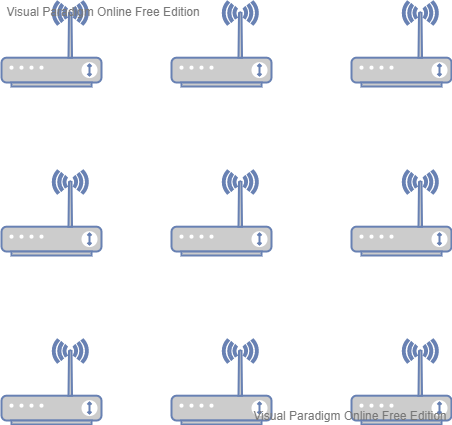
\includegraphics[scale=0.6]{pic1}
\caption{Possible arrangement of nodes}
\label{fig:3}
\end{figure}
\begin{figure}[h]
\centering
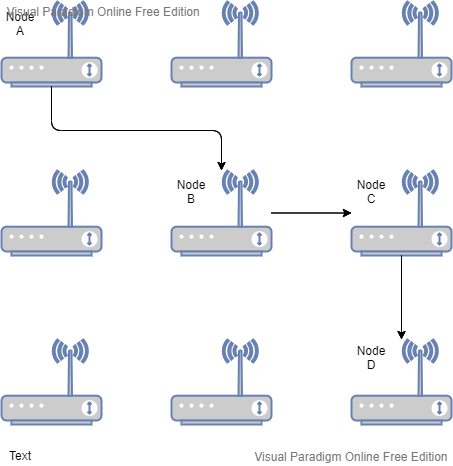
\includegraphics[scale=0.6]{pic2}
\caption{Path from node A to node D, hop-count $=3$}
\label{fig:4}
\end{figure}
\\\\There exists some improvements of the previous algorithm \cite{KAUR201982}, for example the Weighted Centroid Algorithm. Before getting into the formula we need to remind the meaning of hop count. Given a set of connected nodes, the hop count is the number of nodes that the packet goes through before reaching the destination node. For example in the fig \ref{fig:4} node A wants to send a packet to node D, but to do so, the packet need to be relayed by B, then by C and finally it reaches D. The hop count therefore is 3.\\\\
Here we define a new metric as 
\begin{equation}
    w_{u,i}=\frac{1}{h_{u,i}}
\end{equation}
where $h_{u,i}$ is the hop count from node $i$ to the unknown node $u$. The line 4 of the previous algorithm then becomes
\begin{equation}
     x_u=\frac{\sum_{i=1}^mw_{u,i}x_i}{\sum_{i=1}^mw_{u,i}},\quad y_u=\frac{\sum_{i=1}^mw_{u,i}y_i}{\sum_{i=1}^mw_{u,i}}
\end{equation}








\clearpage

\section{DV-Hop Algorithm}
  \begin{center}
  \textbf{Assume to know:}
  \begin{itemize}
    \centering
    \item $\emptyset$
  \end{itemize}
  \end{center}
The DV-Hop algorithm was first published by in \cite{965964}.\\
\begin{algorithm}[H]
\SetAlgoLined
\KwResult{Estimated position of the unknown node}
Each node has built its own database\;
Each node compute the average distance of one hop
\begin{equation}
    AvgHopDistance_i=\frac{\sum_{j=1,j\neq i}^n\sqrt{(x_j-x_i)^2+(y_j-y_i)^2}}{\sum_{j=1,j\neq i}^nh_{i,j}}
\end{equation}\\
The unknown node $u$ computes the approximate distance from anchor node i using 
\begin{equation}
    d_{u,i}=AvgHopDistance_i \cdot h_{u,i}
    \label{eq:19}
\end{equation}
 \caption{DV-Hop algorithm}
\end{algorithm}
\noindent\\
The algorithm begins with a broadcast of all nodes with a packet, that contains informations about its position and the hop count, which starts from zero and it is incremented by one at each node it passes through. Each node upgrade its metrics accordingly. After some time necessary to reach a stable point where no information update happen, we have a situation where every node has the minimum hop count from itself to each node and the positions of each node. For example the following table could be the database stored in node $i$
\begin{center}
\begin{tabular}{ |c|c|c| } 
 \hline
 Node ID & position & hop count \\ 
 \hline
 \hline
 1 & (40,-35) & 6 \\ 
 2 & (-13,18) & 4 \\
 $\hdots$ & $\hdots$ & $\hdots$\\
 \hline
\end{tabular}
\end{center}
As soon as the data is available each unknown node can compute its approximated distance from each node $i $ as in line $3$ of the previous algorithm. Therefore the unknown node $u, 1\leq u\leq n$ is able to derive the following equations (with $x_u,y_u$) unknown
\begin{align}
\begin{split} 
(x_1-x_u)^2+(y_1-y_u)^2&=d_{u,1}^2 \\ 
(x_2-x_u)^2+(y_2-y_u)^2&=d_{u,2}^2 \\ 
&\;\;\vdots\\
(x_n-x_u)^2+(y_n-y_u)^2&=d_{u,n}^2 \\
\end{split}
\end{align} 
where $d_{u,i}$ is the distance (in meters) from node $u$ to node $i$ unknown exactly but estimated as in \ref{eq:19}.
\\\\By subtracting the $n$-th equation to all the others, those can be transformed to
\begin{align}
\begin{split} 
x_1^2-x_n^2+y_1^2-y_n^2-d_{u,1}^2-d_{u,n}^2&=2x_u(x_1-x_n)+2y_u(y_1-y_u)\\ 
x_2^2-x_n^2+y_2^2-y_n^2-d_{u,2}^2-d_{u,n}^2&=2x_u(x_2-x_n)+2y_u(y_2-y_u)\\
&\;\;\vdots\\
x_2^2-x_n^2+y_2^2-y_n^2-d_{u,2}^2-d_{u,n}^2&=2x_u(x_{n-1}-x_n)+2y_u(y_2-y_u)
\end{split}
\end{align}
Can be written in matrix form $\mathbf{Ax}=\mathbf{b}$
where 
\begin{equation}
    \mathbf{A}=2\begin{bmatrix}
    x_1-x_m & y_1-y_m\\
    x_2-x_m & y_2-y_m\\
    \vdots & \vdots\\
    x_{m-1}-x_m & y_{m-1}-y_m
    \end{bmatrix}
\end{equation}
\begin{equation}
    \mathbf{x}=\begin{bmatrix}
    x_u\\
    y_u
    \end{bmatrix}
\end{equation}
\begin{equation}
    \mathbf{b}=\begin{bmatrix}
        x_{1}^2-x_m^2+y_{1}^2-y_m^2-d_{u,1}^2-d^2_{u,m}\\
        x_{2}^2-x_m^2+y_{2}^2-y_m^2-d_{u,2}^2-d^2_{u,m}\\
        \vdots\\
        x_{m-1}^2-x_m^2+y_{m-1}^2-y_m^2-d_{u,n-1}^2-d^2_{u,m}
    \end{bmatrix}
\end{equation}
The result can be computed with the closed formula of the LLS
\begin{equation}
    \mathbf{x}=\mathbf{(A^TA)^{-1}A^Tb}
\end{equation}
\clearpage


\section{Fingerprinting}
  \begin{center}
  \textbf{Assume to know:}
  \begin{itemize}
    \centering
    \item previous $\upsilon_i^j,\forall i,j$
  \end{itemize}
  \end{center}
Fingerprinting \cite{YIU2017235} is a quite general technique, that can be used for many scenarios. Its main drawback is the offline training phase, which needs to be done before the localization takes place, therefore its use is mostly reserved for example for the location of devices in a known area, that can be for example factories, shopping center, where the nodes have all the time to acquire a precise and accurate representation of the normal environment. This comes with a positive side, it is an efficient model-free algorithm, therefore its use is not restricted to signal intensity localization only. As soon as this phase is done, it can start the localization phase. The main principle underlying this method is the analysis of the similarity of signal intensity observed by the unknown node ($u,u>n$) w.r.t. the other nodes. The main principle underlying this method is to compute the squared difference between the signal intensity of all the anchor nodes measured by the unknown node and the signal intensity of all the other nodes measured by each node.
The algorithm employed by this method is known as K-NN or K nearest neighbors \cite{10.5555/1162264}. Here is presented first the version working with 1-NN.
In the learning (offline) phase, each node builds an internal database with records of every node along with the received signal strength as in the the following table (table). As soon as the localization phase starts (computed remotely, since we must have the signal intensity of all the nodes), the following formula is used
\begin{equation}
    \hat{i}=\arg \min_i\bigg\{\sum_{\substack{j=1\\j\neq i}}^n(\upsilon_i^j-\upsilon_{u}^j)^2\bigg\}
\end{equation}
This formula just iterates over all the nodes, and by each node $i$ it computes the difference squared between the intensity of the node $j$ read by the node $i$ ($\upsilon_i^j$) and by the node $u$ ($\upsilon_u^j$) for every node. Clearly, the summation skips the values of equal $i$ and $j$, because it doesn't make sense to measure the intensity of the signal produced by the node itself. Therefore, the node $\hat{i}$ with the minimum sum of square differences, according to the signal intensity read, should be closest to the unknown node. The estimated position is the position of that node. This is a quite raw estimation, since can take only one out of the $n$ known positions, but it can be efficiently improved for higher values of $k$. In those cases, the selected nodes are $k$ instead of one, and the final estimate is computed as the mean of the position of those $k$ nodes, as the name says, the $k$ nearest neighbors.

\chapter{Conclusions}
In this work, I have discussed the main algorithms nowadays available to locate a device with an unknown position through the received signal strength. It is very important to note, however, that those algorithms can be used for the whole class of problems that are based on some path decreasing propagation, regardless of the nature of the signal itself (e.g. sound intensity). Let's take the Quadratic linearization algorithm. Provided you have the mathematical description of the propagation model, and you can derive the distance as in \ref{eq:17}, then the final matrices only depend on the position of the sensing devices and the estimated distances. This reasoning applies also to the other algorithms, clearly the Multilateration algorithm and also the model-free method (possibly with some little adjustments). \\\\
It seems appealing that some algorithms don't require the knowledge of any parameter beforehand. Those are some of the model-free methods and the Multilateration. Regarding the model-free methods, it should be said however that they work well if the anchor nodes are many and regularly positioned (in a grid for example), otherwise the precision downgrades. 
Good results can be obtained with the Fingerprinting method, however, its downside is that it requires a learning phase, where each device measures the intensity read of all the other devices. This reduces the range of applicability of this algorithm. For example, it could not be used generally for disaster response, since there is no physical time to learn the signal intensity of the other nodes. Regarding instead the Multilateration, it could actually work without any previous learning phase nor any parameter but the quality of the estimation degrades. Usually, at least $\upsilon_0$ is required. Additionally, one important drawback is the starting guess. It must be close enough to the real location, otherwise, the method could diverge. A good choice for the starting guess is to use the estimated position from other methods. A good increase in the performance is given by employing an array of custom path loss indexes, different for each anchor node, particularly useful if the location process happens in an environment fitted with obstacles. This improvement comes however with a decrease in performance. \\\\
Optimum results can be obtained when the field of application is well known and the algorithm has all the time required to estimate parameters $\alpha,\sigma_i^2\,\forall i$ with the algorithms presented earlier. In my opinion, the most accurate one would be the Weighted linear estimation, which considers carefully the effect of the variance of the measurements, which is in fact a concise representation of the noise. A particular mention needs to be given also to the line intersection algorithm.\\\\
The use of UAV is spreading more and more in many areas. As a moving anchor node, it could be effectively employed in Multilateration for example, by moving in the area while recording samples as $$(x_i,y_i,\upsilon_i)$$ and then proceed with the usual computation. However it could not be employed in some range free methods, for example the Fingerprinting, since we cannot compare simultaneous measurements in different places.\\\\
As a consequence, it seems that the perfect algorithm doesn't exist, not even a perfect sequence of algorithms. It is a task for the user to choose what fits best its need, based also on his known parameters and his expectations on the accuracy.\\\\











\clearpage
\printbibliography[
heading=bibintoc,
title={Bibliography}
]
%Prints the entire bibliography with the title "Whole bibliography"

%\clearpage

%Filters bibliography
%\printbibliography[heading=subbibintoc,type=article,title={Articles only}]
%\printbibliography[type=book,title={Books only}]
%\printbibliography[keyword={physics},title={Physics-related only}]
%\printbibliography[keyword={latex},title={\LaTeX-related only}]

\end{document}